% =====================================================================
\chapter{Optimización de forma y de topología}
\label{tema:2}
% =====================================================================

La optimización de topología responde a una pregunta de diseño mecánico: dado un volumen de trabajo, unos apoyos, unas cargas y una cantidad de material, ¿dónde se pone el material para que la pieza sea lo más rígida posible? A diferencia de la optimización de forma, que mueve una frontera ya existente, aquí se permite que aparezcan y desaparezcan agujeros. Este tema sigue el capítulo~1 de Bendsøe y Sigmund~\cite{bs}, el artículo de Bendsøe de 1989 que formuló el problema como distribución de material~\cite{bendsoe89}, los códigos didácticos de 99 y 88 líneas~\cite{sigmund99,andreassen}, el estudio de inestabilidades de Sigmund y Petersson~\cite{sigpet} y el análisis de filtros de Bourdin~\cite{bourdin}. El método adjunto se presenta como en las notas de cálculo matricial del MIT~\cite[§6.3]{mit18s096}.

\section{El problema de flexibilidad mínima}

Se discretiza el dominio de diseño en $N$ elementos finitos cuadrados. El elemento $e$ tiene una densidad $x_e\in[0,1]$ (0 vacío, 1 material) y una matriz de rigidez $E_e\,k_0$, donde $k_0\in\R^{8\times 8}$ es la del elemento bilineal con módulo unidad. El ensamblado da la matriz global $K(x)=\sum_e E_e(x_e)\,P_e^\T k_0P_e$, simétrica y definida positiva una vez impuestos los apoyos, donde $P_e$ extrae los ocho grados de libertad del elemento.

\begin{definicion}[Flexibilidad mínima con restricción de volumen]\label{def:compliance}
Dadas las cargas $F$ y una fracción de volumen $f_V\in(0,1)$, el problema es
\[
\min_{x\in[0,1]^N}\ c(x)=F^\T U(x)\quad\text{sujeto a}\quad K(x)\,U(x)=F,\qquad \frac1N\sum_{e=1}^N x_e=f_V .
\]
La \emph{flexibilidad} $c=F^\T U=U^\T KU$ es el trabajo de las cargas exteriores, igual al doble de la energía elástica almacenada; minimizarla equivale a maximizar la rigidez global.
\end{definicion}

Si las densidades solo pudieran valer 0 o 1, el problema sería combinatorio, con $2^N$ diseños. La relajación a $[0,1]$ lo vuelve continuo y derivable, pero entonces hay que conseguir que el óptimo no esté lleno de material «gris» de densidad intermedia, que no se puede fabricar.

\section{La interpolación SIMP}

\begin{definicion}[SIMP modificado]\label{def:simp}
El método SIMP (\emph{solid isotropic material with penalization}) interpola el módulo de Young como
\[
E_e(x_e)=\Emin+x_e^{\,p}\,(E_0-\Emin),\qquad p>1,
\]
con $\Emin>0$ pequeño (por ejemplo $10^{-9}E_0$) para que $K$ no sea singular cuando hay elementos vacíos~\cite[§2.1]{andreassen}.
\end{definicion}

La penalización funciona porque el volumen es lineal en $x_e$ y la rigidez no. Con $p=3$, un elemento a densidad $0{,}5$ consume la mitad del material pero aporta solo $0{,}5^3=0{,}125$ de la rigidez: la relación rigidez/volumen es $x_e^{p-1}=0{,}25$, cuatro veces peor que la del material sólido. El optimizador aprende así a evitar los grises. El precio es la pérdida de convexidad.

\begin{teorema}[Convexidad con $p=1$]\label{teo:convexo}
Si $E_e(x_e)=\Emin+x_e(E_0-\Emin)$, es decir, con $p=1$, la flexibilidad $c(x)=F^\T K(x)^{-1}F$ es una función convexa de $x$ en $[0,1]^N$.
\end{teorema}

\begin{proof}
Para una matriz $K$ simétrica definida positiva se cumple
\[
F^\T K^{-1}F=\max_{u}\ \bigl(2F^\T u-u^\T Ku\bigr),
\]
porque la función de $u$ entre paréntesis es cóncava, su gradiente $2F-2Ku$ se anula en $u=K^{-1}F$ y su valor ahí es $2F^\T K^{-1}F-F^\T K^{-1}F=F^\T K^{-1}F$. Con $p=1$, $K(x)$ es afín en $x$, así que para cada $u$ fijo la función $x\mapsto 2F^\T u-u^\T K(x)u$ es afín. El máximo puntual de una familia de funciones afines es convexo (módulo~4, tema~5), luego $c$ es convexa.
\end{proof}

Con $p=1$ (la «chapa de espesor variable») el problema es convexo y su óptimo global es fácil de alcanzar, pero contiene grandes zonas grises. Con $p=3$, el valor estándar, desaparece la convexidad y el resultado depende del punto de partida y de los parámetros; el filtrado y las estrategias de continuación en $p$ mitigan el problema~\cite{sigpet}.

\section{Sensibilidades por el método adjunto}

\begin{teorema}[Método adjunto para ecuaciones de equilibrio]\label{teo:adjunto}
Sea $J(x)=g\bigl(x,U(x)\bigr)$ con $K(x)U=F$, $K(x)$ invertible y derivable, y $F$ independiente de $x$. Sea $\lambda$ la solución del \emph{problema adjunto} $K(x)^\T\lambda=\bigl(\partial g/\partial U\bigr)^\T$. Entonces
\[
\frac{dJ}{dx_e}=\frac{\partial g}{\partial x_e}-\lambda^\T\frac{\partial K}{\partial x_e}\,U .
\]
\end{teorema}

\begin{proof}
Derivando $KU=F$ respecto a $x_e$ se obtiene $\frac{\partial K}{\partial x_e}U+K\frac{dU}{dx_e}=0$, luego $\frac{dU}{dx_e}=-K^{-1}\frac{\partial K}{\partial x_e}U$. Por la regla de la cadena,
\[
\frac{dJ}{dx_e}=\frac{\partial g}{\partial x_e}+\frac{\partial g}{\partial U}\frac{dU}{dx_e}=\frac{\partial g}{\partial x_e}-\frac{\partial g}{\partial U}K^{-1}\frac{\partial K}{\partial x_e}U .
\]
Agrupando de izquierda a derecha, $\frac{\partial g}{\partial U}K^{-1}=\lambda^\T$ con $K^\T\lambda=(\partial g/\partial U)^\T$, y queda la fórmula.
\end{proof}

La demostración es la asociatividad del producto de jacobianos que distingue el modo inverso del directo (módulo~10, §4.2): multiplicar primero $\frac{\partial g}{\partial U}K^{-1}$ cuesta una sola resolución, sea cual sea el número $N$ de variables, mientras que calcular cada $dU/dx_e$ costaría $N$ resoluciones. El vector $\lambda$ es el multiplicador de Lagrange de la restricción $KU=F$ (módulo~10, §5.4).

\begin{corolario}[La flexibilidad es autoadjunta]\label{cor:autoadjunto}
Para $c=F^\T U$ se tiene $\lambda=U$ y
\[
\frac{\partial c}{\partial x_e}=-U^\T\frac{\partial K}{\partial x_e}U=-p\,x_e^{\,p-1}(E_0-\Emin)\,u_e^\T k_0u_e\ \le 0 .
\]
\end{corolario}

\begin{proof}
$g=F^\T U$ no depende explícitamente de $x$ y $(\partial g/\partial U)^\T=F$, luego el problema adjunto es $K\lambda=F$ ($K$ es simétrica), cuya solución es $U$. Además $\partial K/\partial x_e=p\,x_e^{p-1}(E_0-\Emin)P_e^\T k_0P_e$, y $U^\T P_e^\T k_0P_eU=u_e^\T k_0u_e\ge 0$ porque $k_0$ es semidefinida positiva.
\end{proof}

El signo tiene una lectura física: añadir material nunca hace la estructura más flexible. Calcular el gradiente completo no cuesta ninguna resolución adicional; basta con la energía $u_e^\T k_0u_e$ de cada elemento.

\begin{ejemplo}[Dos barras en serie]\label{ej:serie}
Dos barras en serie, con rigideces $k_e=x_e^{3}k_0$ ($k_0=1000$ N/mm), densidades $x=(0{,}8;\ 0{,}5)$ y carga $F=100$ N en el extremo libre. Entonces $k=(512;\ 125)$ N/mm y $c=F^2(1/k_1+1/k_2)=10^4(0{,}001953+0{,}008)=99{,}53$ N·mm. Los alargamientos son $u_e=F/k_e$, y por el \cref{cor:autoadjunto},
\[
\frac{\partial c}{\partial x_e}=-3x_e^2k_0\,u_e^2=-\frac{3x_e^2k_0F^2}{k_e^2}:\qquad \frac{\partial c}{\partial x_1}=-73{,}24,\quad \frac{\partial c}{\partial x_2}=-480\ \ \text{N·mm}.
\]
Con el mismo material añadido, la barra débil reduce la flexibilidad 6,6 veces más: la sensibilidad indica dónde se necesita el material.
\end{ejemplo}

\section{Actualización por criterios de optimalidad}

Con $V(x)=\sum_ev_ex_e$ (en la malla regular, $v_e=1$), la lagrangiana del problema es $c(x)+\Lambda\bigl(V(x)-Nf_V\bigr)$ más los términos de las cotas. Para un elemento con $0<x_e<1$, la condición de estacionariedad (0.7, §5.4) es $-\partial c/\partial x_e=\Lambda\,v_e$, es decir,
\[
B_e:=\frac{-\partial c/\partial x_e}{\Lambda\,\partial V/\partial x_e}=1 .
\]
La actualización por criterios de optimalidad (OC) convierte esta condición en una iteración de punto fijo: si $B_e>1$, el elemento rinde más que el precio $\Lambda$ del material y conviene aumentar $x_e$; si $B_e<1$, disminuirla.

\begin{definicion}[Actualización OC]\label{def:oc}
Con amortiguamiento $\eta=1/2$ y límite de movimiento $m$ (0,2 en~\cite{andreassen}),
\[
x_e^{\text{nuevo}}=\clip\Bigl(x_eB_e^{\eta},\ \max(0,x_e-m),\ \min(1,x_e+m)\Bigr),
\]
donde $\Lambda$ se elige por bisección para que $x^{\text{nuevo}}$ cumpla la restricción de volumen.
\end{definicion}

\begin{proposicion}\label{prop:biseccion}
Si $\partial c/\partial x_e<0$ para todo $e$, el volumen $V\bigl(x^{\text{nuevo}}(\Lambda)\bigr)$ es una función continua y no creciente de $\Lambda>0$; por tanto, la bisección encuentra un $\Lambda$ que cumple la restricción siempre que esta sea alcanzable dentro de los límites de movimiento.
\end{proposicion}

\begin{proof}
$B_e^\eta=\bigl(-\partial_ec/(\Lambda v_e)\bigr)^{\eta}$ es continua y estrictamente decreciente en $\Lambda$, la función $\clip$ es continua y no decreciente en su primer argumento, y $V$ es una suma con coeficientes positivos. Una función continua y monótona que toma valores por encima y por debajo del objetivo en los extremos del intervalo de búsqueda alcanza el objetivo (teorema de Bolzano), y la bisección lo localiza.
\end{proof}

\section{Inestabilidades numéricas y filtros}

Sin regularización, SIMP produce dos patologías bien documentadas~\cite{sigpet}: \emph{tableros de ajedrez}, zonas de elementos sólidos y vacíos alternados que el elemento bilineal considera artificialmente rígidas, y \emph{dependencia de la malla}: al refinar aparecen cada vez más barras finas, porque el problema continuo carece de solución con microestructura acotada. La solución estándar es imponer una escala de longitud mínima mediante un filtro de radio $\rmin$, con pesos
\[
H_{ei}=\max\bigl(0,\ \rmin-\operatorname{dist}(e,i)\bigr),
\]
donde la distancia se mide entre centros de elementos.

\begin{definicion}[Filtros de sensibilidades y de densidades]\label{def:filtros}
El \emph{filtro de sensibilidades}~\cite{sigmund99,andreassen} sustituye las derivadas por un promedio ponderado,
\[
\widehat{\frac{\partial c}{\partial x_e}}=\frac{1}{\max(\gamma,x_e)\sum_iH_{ei}}\sum_iH_{ei}\,x_i\,\frac{\partial c}{\partial x_i},\qquad \gamma=10^{-3}.
\]
El \emph{filtro de densidades}~\cite{bourdin} define densidades físicas $\xf_e=\sum_iH_{ei}x_i/\sum_iH_{ei}$, con las que se calcula la rigidez; las sensibilidades respecto a las variables de diseño se obtienen por la regla de la cadena,
\[
\frac{\partial c}{\partial x_j}=\sum_e\frac{\partial c}{\partial\xf_e}\frac{\partial\xf_e}{\partial x_j}=\sum_e\frac{H_{ej}}{\sum_iH_{ei}}\,\frac{\partial c}{\partial\xf_e}.
\]
\end{definicion}

El filtro de densidades tiene una justificación matemática: Bourdin demuestra que el problema filtrado tiene solución y que las aproximaciones por elementos finitos convergen~\cite{bourdin}. El filtro de sensibilidades es heurístico (el gradiente filtrado no es el de ninguna función), pero funciona muy bien en la práctica. En ambos casos, el diseño que se presenta es el de las densidades físicas $\xf$, no el de las variables $x$~\cite[§2.3]{andreassen}. La proyección de Heaviside, $\bar x=1-e^{-\beta\xf}+\xf e^{-\beta}$ con $\beta$ creciente, elimina los grises que el filtro de densidades deja en los bordes.

\section{Caso de estudio: la viga MBB}

\begin{ejemplo}[Viga MBB con el código de 88 líneas en numpy]\label{ej:mbb}
\emph{Problema.} La viga MBB es una viga biapoyada con una carga puntual en el centro del borde superior. Por simetría se modela la mitad: un dominio de $60\times 20$ elementos cuadrados de 1 mm, con los desplazamientos horizontales impedidos en el borde izquierdo (eje de simetría), el vertical impedido en la esquina inferior derecha (apoyo) y una carga vertical unitaria en la esquina superior izquierda. Fracción de volumen $f_V=0{,}5$, $p=3$, $E_0=1$, $\Emin=10^{-9}$, $\nu=0{,}3$, filtro de sensibilidades con $\rmin=2{,}4$ ($0{,}04$ veces la anchura, como en los ensayos de~\cite[§3.4]{andreassen}).

\emph{Formulación.} La de la \cref{def:compliance} con SIMP, $N=1200$ variables y $2\cdot 61\cdot 21=2562$ grados de libertad. En cada iteración: (1) ensamblar $K(\xf)$ en formato disperso; (2) resolver $KU=F$; (3) calcular $u_e^\T k_0u_e$ y las sensibilidades del \cref{cor:autoadjunto}; (4) filtrar; (5) actualizar con OC (\cref{def:oc}). Se para cuando el cambio máximo de densidad es menor que 0,01.

\emph{Elección del método.} Las sensibilidades adjuntas cuestan cero resoluciones adicionales; por diferencias finitas, cada iteración necesitaría 1201 resoluciones. OC es el método más simple para un problema con una única restricción y gradientes de signo conocido (\cref{prop:biseccion}); con varias restricciones se usa el método de las asíntotas móviles (MMA).

\emph{Resultado.} La traducción a numpy y scipy del código de Andreassen \emph{et al.} converge en 106 iteraciones (unos 1,6 s en una CPU) a una flexibilidad $c=216{,}81$, el valor publicado en~\cite[fig.~3]{andreassen}; la flexibilidad inicial con densidad uniforme era $1007{,}0$, de modo que la optimización la reduce un 78~\%. Con filtro de densidades se obtiene $c=233{,}71$, también idéntico al publicado, en 144 iteraciones, y un diseño con bordes más difusos (\cref{fig:mbb}): la medida de grises $4\,\overline{\xf(1-\xf)}$ vale $0{,}265$ con el filtro de sensibilidades y $0{,}330$ con el de densidades. Con la llamada por defecto del artículo, $\rmin=1{,}5$, la flexibilidad baja a $203{,}19$ porque se permiten barras más finas.

\emph{Unidades físicas.} Para elementos cuadrados en tensión plana, $K$ escala con $E_0t$ ($t$ espesor) y no depende del tamaño del elemento, así que $c_{\text{fís}}=\bar c\,F^2/(E_0t)$. Con aluminio ($E_0=70$ GPa), $t=10$ mm y $F=1$ kN en el semimodelo (2 kN sobre la viga completa de $120\times 20$ mm): $c_{\text{fís}}=216{,}81\cdot 10^6/(7\cdot 10^{8})=0{,}310$ J, flecha bajo la carga $c/F=0{,}310$ mm y masa del semimodelo $0{,}5\cdot 60\cdot 20\cdot 10$ mm³ $\cdot\,2{,}70$ g/cm³ $=16{,}2$ g.
\end{ejemplo}

\begin{figure}[h]
\centering
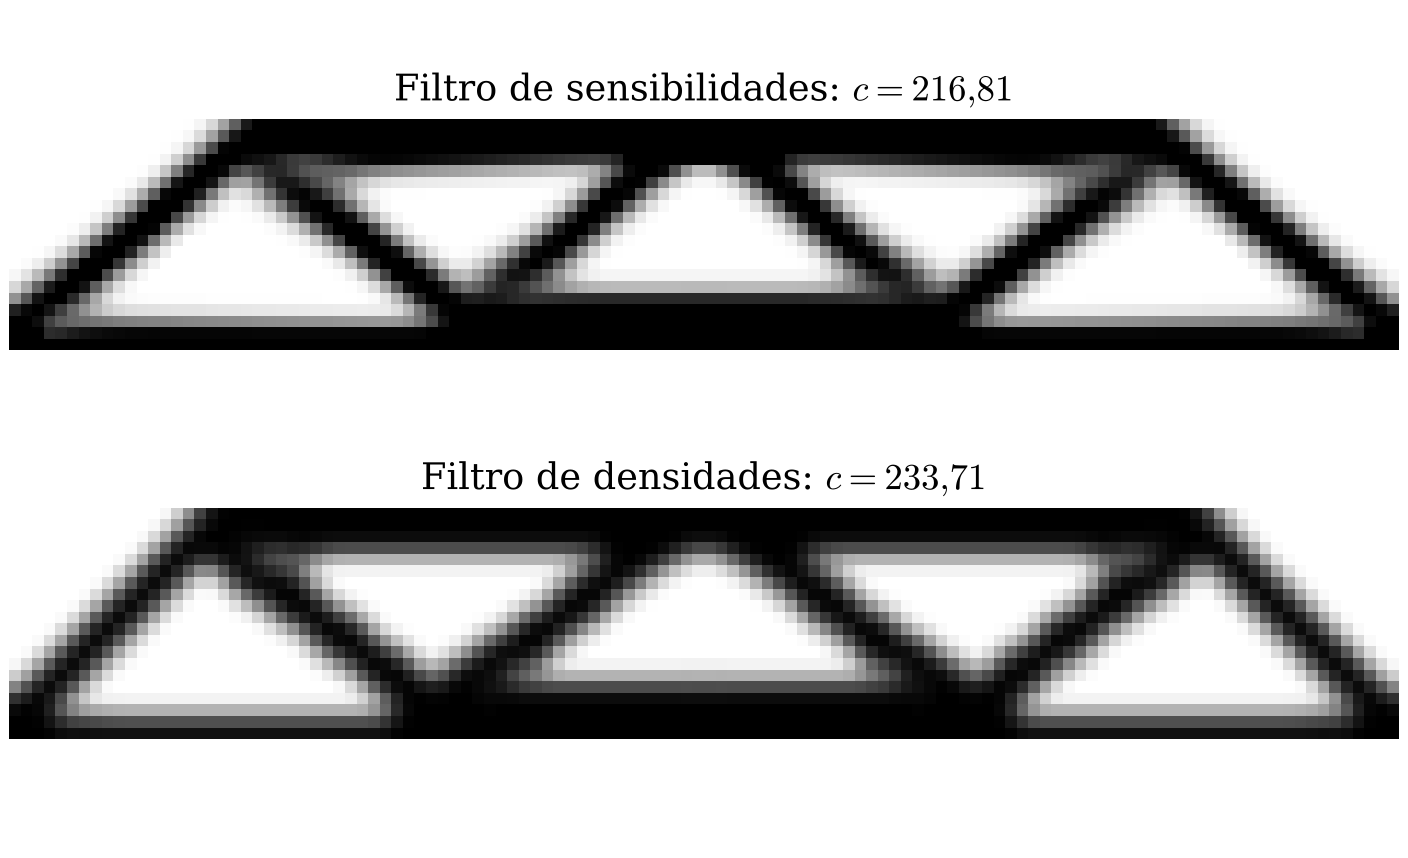
\includegraphics[width=0.82\textwidth]{fig-mbb.png}
\caption{Diseños de la viga MBB completa (semimodelo de $60\times 20$ elementos reflejado), $f_V=0{,}5$, $p=3$, $\rmin=2{,}4$. Negro: material. Calculado con el cuaderno del módulo.}
\label{fig:mbb}
\end{figure}

\section{Fabricación aditiva y diseño generativo}

Un diseño optimizado solo es útil si se puede fabricar. Las restricciones más comunes son el tamaño mínimo de las barras y de los huecos, que el radio del filtro controla; la dirección de fabricación, porque en fabricación aditiva las superficies que miran hacia abajo con poca inclinación necesitan soportes (\cref{tema:6}); y, para mecanizado o fundición, la accesibilidad de la herramienta y el desmoldeo. Langelaar propuso un filtro que, capa a capa, solo permite material que esté sostenido por material de la capa inferior, de modo que el resultado es imprimible sin soportes~\cite{langelaar}. Tras optimizar, el flujo habitual es umbralizar $\xf$, extraer la superficie (\emph{marching cubes} o \emph{squares}, \cref{tema:1}), suavizarla, reconstruir una geometría CAD y \emph{volver a verificar} con un análisis de elementos finitos más fino, incluyendo tensiones, que el problema de flexibilidad no controla.

Los programas comerciales de \emph{diseño generativo} empaquetan este flujo. La documentación pública de Autodesk Fusion describe métodos de fabricación seleccionables (sin restricciones, aditiva con dirección de impresión, fresado de 2,5, 3 y 5 ejes, corte en 2 ejes y fundición con espesor mínimo, ángulo de desmoldeo y dirección de expulsión), cada uno de los cuales genera su propio conjunto de resultados~\cite{fusiongd}. El caso publicado más citado es el soporte de cinturón de un asiento de General Motors: según Autodesk, el diseño generativo consolidó ocho piezas en una sola de acero inoxidable, un 40~\% más ligera y un 20~\% más resistente que la anterior~\cite{gmautodesk}. nTop combina el modelado implícito con resultados de optimización de topología y con campos que modulan celosías y espesores~\cite{ntop}. No se han publicado los algoritmos internos de estos productos.

\begin{table}[h]
\centering\small
\begin{tabularx}{\textwidth}{@{}l>{\raggedright\arraybackslash}X>{\raggedright\arraybackslash}p{2.7cm}>{\raggedright\arraybackslash}X@{}}
\toprule
Herramienta & Para qué sirve & Licencia o tipo & Cuándo elegirla \\
\midrule
top88 y variantes (DTU) & códigos didácticos SIMP en MATLAB & descarga gratuita (DTU) & aprender y prototipar en 2D \\
numpy + scipy.sparse & montaje y resolución de elementos finitos & BSD & reproducir top88 en Python (cuaderno) \\
NLopt (MMA) & optimización con muchas restricciones & MIT & sustituir OC cuando hay varias restricciones \\
dolfin-adjoint & adjuntos automáticos sobre FEniCS & LGPL & EDP generales en 2D y 3D sin derivar a mano \\
Autodesk Fusion & diseño generativo con restricciones de fabricación & comercial & ingeniería de producto con CAD integrado \\
nTop & modelado implícito, celosías, campos & comercial & piezas para fabricación aditiva con celosías \\
\bottomrule
\end{tabularx}
\caption{Tecnologías del tema~2.}
\label{tab:tec2}
\end{table}

\begin{observacion}[Errores frecuentes en la práctica]\label{obs:errores2}
(i) \emph{No filtrar}: aparecen tableros de ajedrez y el resultado depende de la malla. (ii) \emph{Presentar $x$ en lugar de $\xf$} con el filtro de densidades: el diseño mostrado no es el analizado. (iii) \emph{$\Emin=0$}: $K$ se vuelve singular en cuanto un elemento se vacía. (iv) \emph{Confundir rigidez con resistencia}: mínima flexibilidad no garantiza tensiones admisibles; hay que comprobarlas, sobre todo en esquinas entrantes. (v) \emph{Mínimos locales}: con $p=3$ el resultado depende de los parámetros; conviene la continuación en $p$ y comparar varias ejecuciones. (vi) \emph{Olvidar la fabricación}: voladizos, cavidades cerradas que atrapan polvo o resina y espesores inferiores a la resolución de la máquina. (vii) \emph{Coste}: en 3D, la resolución de $KU=F$ domina; se necesitan resolvedores iterativos con precondicionadores multimalla para pasar de unos miles a millones de elementos.
\end{observacion}

\begin{lecturas}
\item M.~P. Bendsøe y O.~Sigmund~\cite{bs}, cap.~1 «Topology optimization by distribution of isotropic material».
\item E.~Andreassen \emph{et al.}~\cite{andreassen}: §2 (formulación, SIMP modificado, OC y filtros) y §3 (implementación).
\item O.~Sigmund y J.~Petersson~\cite{sigpet}: tableros de ajedrez, dependencia de la malla y mínimos locales.
\item P.~Bright, A.~Edelman y S.~G. Johnson~\cite{mit18s096}, §6.3 «Reverse-mode “adjoint” differentiation».
\item M.~Langelaar~\cite{langelaar}: restricciones de voladizo para fabricación aditiva.
\end{lecturas}

\section*{Ejercicios del tema 2}
\addcontentsline{toc}{section}{Ejercicios del tema 2}

\begin{ejercicio}{1}{eje:2-vf}
Justifique si son verdaderas o falsas: (a) con $p=1$ el diseño óptimo suele ser blanco y negro; (b) $\Emin>0$ evita que $K$ sea singular; (c) minimizar la flexibilidad equivale a minimizar la flecha en todos los puntos; (d) el filtro de sensibilidades calcula el gradiente exacto de una función filtrada.
\end{ejercicio}

\begin{ejercicio}{1}{eje:2-gd}
Explique por qué el resultado de un programa de diseño generativo debe volver a analizarse por elementos finitos antes de fabricarlo, y cite dos comprobaciones que el problema de flexibilidad mínima no incluye.
\end{ejercicio}

\begin{ejercicio}{2}{eje:2-penal}
Para $x_e=0{,}5$, calcule la relación rigidez/volumen $E_e/(E_0x_e)$ con $p=1,2,3$ ($\Emin\approx 0$). ¿Qué densidad necesita un elemento con $p=3$ para aportar la mitad de la rigidez del sólido?
\end{ejercicio}

\begin{ejercicio}{2}{eje:2-oc}
Tres elementos con $x=(0{,}5;\ 0{,}5;\ 0{,}5)$, sensibilidades $\partial c/\partial x=(-4;\ -1;\ -0{,}25)$, $\partial V/\partial x_e=1$, $\eta=1/2$, $m=0{,}2$ y volumen objetivo $1{,}5$. Aplique la \cref{def:oc} y encuentre el valor de $\Lambda$ que cumple el volumen.
\end{ejercicio}

\begin{ejercicio}{2}{eje:2-filtro}
En una malla regular con $\rmin=1{,}5$ y densidades uniformes $x_i=0{,}5$, el elemento central de un bloque $3\times 3$ tiene sensibilidad $-4$; sus cuatro vecinos laterales, $-2$, y sus cuatro vecinos diagonales, $-1$. Calcule la sensibilidad filtrada del elemento central.
\end{ejercicio}

\begin{ejercicio}{2}{eje:2-cadena}
Una fila de tres elementos con $\rmin=1{,}5$ (peso propio $1{,}5$ y peso $0{,}5$ para los vecinos inmediatos) y $x=(1;\ 0{,}5;\ 0)$. Calcule las densidades físicas $\xf$ y, si $\partial c/\partial\xf=(-3;\ -2;\ -1)$, las sensibilidades respecto a $x$. Compruebe que la suma de sensibilidades se conserva.
\fuente{adaptado de IUPUI ME 60602 «Topology Optimization» (A.~Tovar), clase~12 «Well-posedness, numerical problems, filters»~\cite{tovar}.}
\end{ejercicio}

\begin{ejercicio}{2}{eje:2-fisico}
El resultado adimensional $\bar c=216{,}81$ de la viga MBB se fabrica en acero ($E_0=200$ GPa, densidad $7{,}85$ g/cm³) con espesor $t=5$ mm, elementos de 1 mm y una carga de 2 kN en el semimodelo. Calcule la flexibilidad física, la flecha bajo la carga y la masa del semimodelo.
\end{ejercicio}

\begin{ejercicio}{3}{eje:2-mecanismo}
En un mecanismo flexible se quiere maximizar el desplazamiento de un nodo de salida, $g=L^\T U$, con $L$ el vector canónico de ese grado de libertad. (a) Escriba el problema adjunto y la sensibilidad $dg/dx_e$ con el \cref{teo:adjunto}. ¿Cuántas resoluciones cuesta el gradiente? (b) Compruébelo en el sistema de dos muelles en serie del \cref{ej:serie} tomando como salida el nodo intermedio, $g=u_1$, cuyo valor exacto es $F/k_1$.
\fuente{adaptado de MIT 18.S096 «Matrix Calculus for Machine Learning and Beyond» (A.~Edelman y S.~G. Johnson, IAP 2023), §6.3 «Reverse-mode “adjoint” differentiation»~\cite{mit18s096}.}
\end{ejercicio}

\begin{ejercicio}{3}{eje:2-kkt}
(a) Demuestre que en el problema de la \cref{def:compliance} con SIMP se cumple $\partial c/\partial x_e\le 0$ y deduzca que en un óptimo con $0<x_e<1$ para algún $e$ la restricción de volumen puede tomarse como desigualdad activa $\sum_ex_e\le Nf_V$. (b) Escriba las condiciones de Karush--Kuhn--Tucker con las cotas $0\le x_e\le 1$ y deduzca que, para los elementos interiores, $B_e=1$, y que en los elementos con $x_e=1$ se cumple $B_e\ge 1$.
\fuente{adaptado de M.~P. Bendsøe y O.~Sigmund, \emph{Topology Optimization}, cap.~1~\cite{bs}.}
\end{ejercicio}
